\documentclass[letterpaper, 10pt,titlepage]{article}

\usepackage{graphicx}                                        
\usepackage{amssymb}                                         
\usepackage{amsmath}                                         
\usepackage{amsthm}                                          
\usepackage{alltt}                                           
\usepackage{float}
\usepackage{color}
\usepackage{url}
\usepackage{pst-gantt}
\usepackage[letterpaper, margin=0.75in]{geometry}
\usepackage{balance}
\usepackage[TABBOTCAP, tight]{subfigure}
\usepackage{enumitem}
\usepackage{pstricks, pst-node}
\usepackage{hyperref}
\usepackage[utf8]{inputenc}
\usepackage{underscore}
 \usepackage{url}
\hypersetup{
  colorlinks = true,
  linkcolor  = black
}

\setcounter{secnumdepth}{4}
\def\name{Chongxian Chen}

\hypersetup{
  colorlinks = true,
  urlcolor = black,
  pdfauthor = {\name},
  pdfkeywords = {Problem Statement},
  pdftitle = {Capstone Project},
  pdfsubject = {Capstone Project},
  pdfpagemode = UseNone
}

\renewcommand*\contentsname{Table of Contents}


\begin{document}

\begin{center}

Oregon State University Computer Science Senior Design
\bigbreak
Progress Report Winter 2017
\bigbreak
By Chen Chongxian
\bigbreak
Team Name: Stat Champs
\bigbreak
\vspace{3.0cm}
Abstract
\bigbreak
\
The application of machine learning to Biochemistry and Biophysics has enabled researchers in this field to make remarkable discoveries, such as the generation of new DNA sequences. However, students of Biochemistry and Biophysics do not get the opportunity to learn machine learning. Dr. Victor Hsu of the Oregon State University Biochemistry and Biophysics department has commissioned the Stat Champs to produce an instructional module to give his students the chance to familiarize themselves with machine learning. The software product the Stats Champs have agreed to develop is a web page that allows students to train a machine learning model based on the college basketball statistics and machine learning algorithm of their choosing in order to produce a March Madness bracket. This will help students understand how machine learning algorithms produce models and how inclusion or exclusion of certain data can influence such models. Over the course of Fall term 2016, the Stat Champs have developed materials such as design documents and technology reviews in order to prepare for the engineering of this module. This report comprehensively describes the progress the Stat Champs have made thus far. For the course of Winter term 2017, the Stat Champs have 
\newpage
\end{center}

\tableofcontents

\newpage
\section{Introduction}
\
\par This report chronicles the progress the author have made on developing the machine learning instructional tool. As of the end of Winter term 2017, I have completed all three responsibility of mine. I made the python script that build a model from previous NCAA basketball matches and then use this model to predict March Madness result of season 2017. The output includes a CSV file prediction and a more readable March Madness tourney bracket picture. My python script also allows the users to choose different stats they want to consider in this prediction and thus fulfill the requirement from our client Dr.Hsu for making this project educational for his students. I also made a simple php table so we have a basic GUI to allow users easily use my python script and see the results.



\section{Chongxian Chen's progress in Winter 2017}
\

\par In week 1 we have our first meeting in Winter term. We agreed on a weekly meeting time with our TA and talked about progress over the break. We are going to start implementing our plan soon. We look forward to a great term.

\par In week 2 we planned what we want to accomplish before midterm. I have started on trying to use support vector machine to classify the the game results. Next I will supply the model with two to three variables and see which SVM core I should use to get more accurate results.

\par In week 3 Jake collect some data. I used excel to convert the file into csv file. The data includes the stats for more than 300 schools in NCAA including detailed data such as field goal and field goal percentage. The data will be great to use as training set. We will also be needing single match data and result to be both as training set and test set for our classification model. Since single match with result will have a true(win)/false(loss) result that we can verify the accuracy of our model.
The difficulty I have in this week is trying to understand the mathematical background of classification model. And what file format to save our data. With our TA's help, I figured that both .txt and .csv file will be sufficient to save the data.
Next week we will collect more data includes single matches in NCAA and use scikit to train and test the model.

\par In week 4 Jake collected a lot of data for NCAA matches. And after learning from classification examples I was able to read all the csv data file successfully into numpy array. I also tried using sklearn to train the model and produce a test outcome. The outcome basically looks fitting to the data, i.e the predicted outcome relates to the expected outcome mostly correct. But the prediction also generate some extreme confidence like 99 percent of winning chance. Which I think could be problematic since extreme prediction will have a extreme penalty in LogLoss equation. We will need to be more careful with extreme prediction. Next week I will look into the extreme prediction in more detail to make our predictions more reasonable.

\par In week 5 our team are working toward our alpha release. After generating the output, I start to analyze the output with LogLoss formula and test multiple different classifiers. I also tried to use different training data sets and testing data sets to see different output. Next week we will finish up our alpha release.

\par In week 6 we got together to write our progress report. We also creates our slides for presentation and record a presentation mp4 file together. We didn't have too much difficulties as we have done something similar last term. Next week we will be continuing improving our project and finish other responsibilities of our project.\par In week 1 we have our first meeting in Winter term. We agreed on a weekly meeting time with our TA and talked about progress over the break. We are going to start implementing our plan soon. We look forward to a great term.

\par In week 7 Last week we finished our alpha release this week I am working on how to make our predictions more accurate. I research about March Madness competition to have a better understanding and also read some data analysis visualization techniques to help me better understand which attribute of our basketball data may play a big part in the match outcome. Next week we will prepare for our beta release.


\par In week 8 After releasing our alpha release, we are working on our beta release which includes integrating machine learning into the website, enhancing machine learning algorithm and allowing the users to choose different categories they want. I have made progress in enhancing the algorithm and we still need to meet together and think about integrating it into the website since none of us have previous experience integrating python script with the website. We will be working on it next week and have our presentation next Friday.

\par In week 9 we had a short presentation of our project on Thursday morning. After having the python script, I am working on allowing the users to select different stats they want to consider in this March Madness prediction. I figured that will be reliable using python command line tools since that will make our future work in websites easier. Then I wrote the php that have a simple table allowing the users to choose stats, and put the user's choice array into the python command line, generate the csv file. Finally use a bracket generator to generate a user-friendly picture. At this point I am basically done with my three responsibilities.

\par During the fianls week we finished our voice over presentation and summarized our term progress report. The recording and editing goes smoothly. We are looking forward to the Spring Expo.

\section{Retrospective}
\begin{center}
    \begin{tabular}{ | l | l | p{3cm} |}
    \hline
    Positives & Deltas & Actions \\ \hline
    Finished required responsibilities & AWS server is too slow & Upgrade AWS machine for a better server \\ \hline

    Made our poster draft & Need to improve Expo presentation skills & Will practice presentation during Spring \\ \hline
    \end{tabular}
\end{center}

\section{Screenshots of the results}
\graphicspath{ {images/} }

\par
\subsection{A table written in php that allows the user to choose different stats to be considered in the prediction.}
\bigbreak
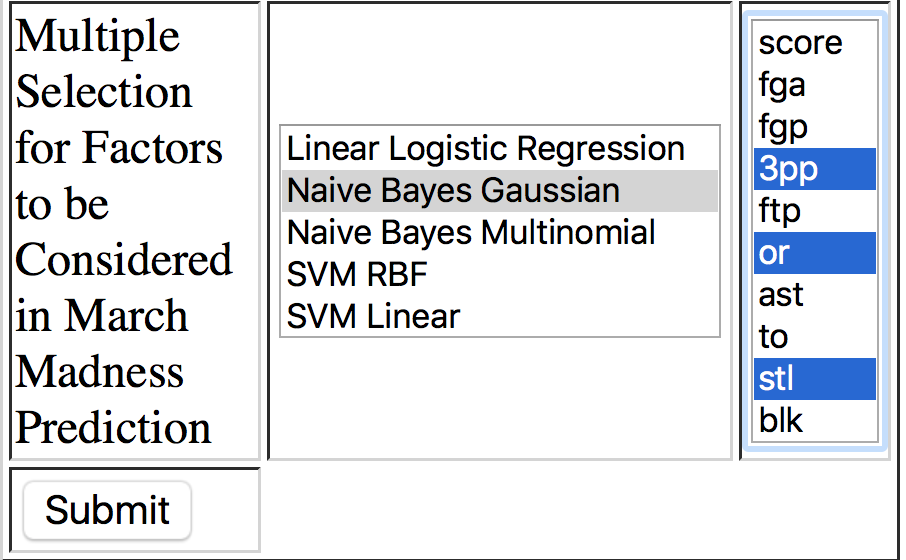
\includegraphics[width=0.5\textwidth]{table.png}

\subsection{Output of the python script generating the results from the user's choice.}
\bigbreak
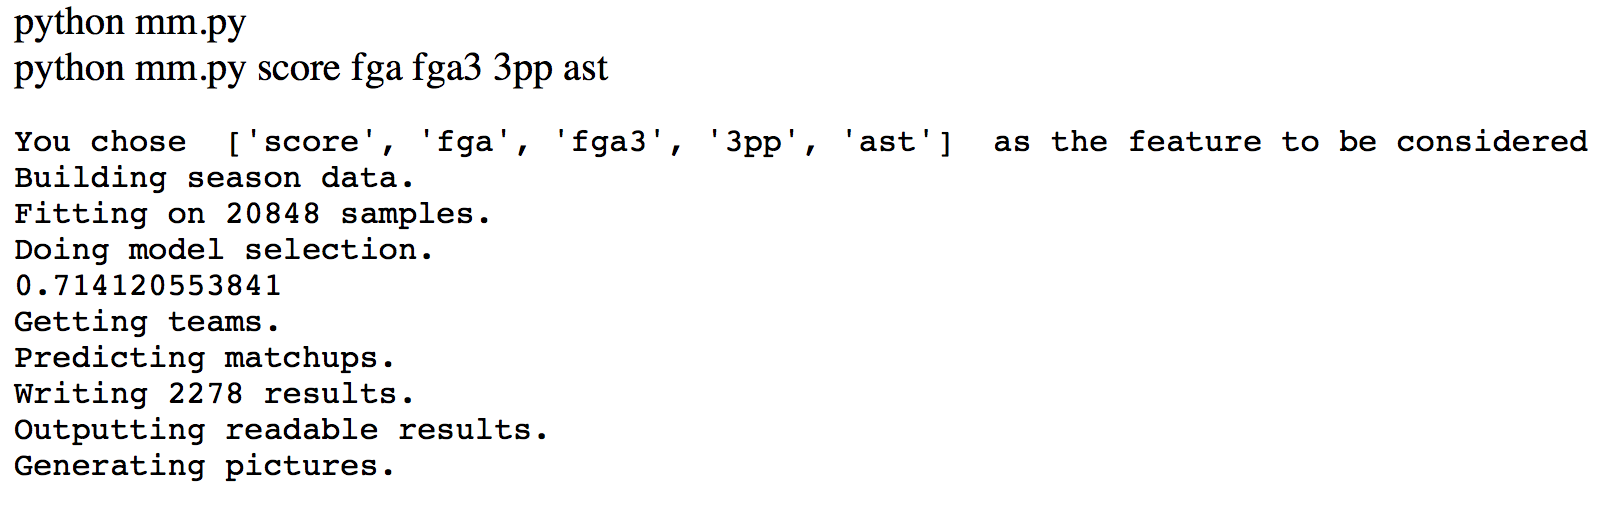
\includegraphics[width=0.8\textwidth]{result.png}

\newpage
\subsection{ A bracket that uses March Madness 2017 format and shows the prediction from our model}
\bigbreak
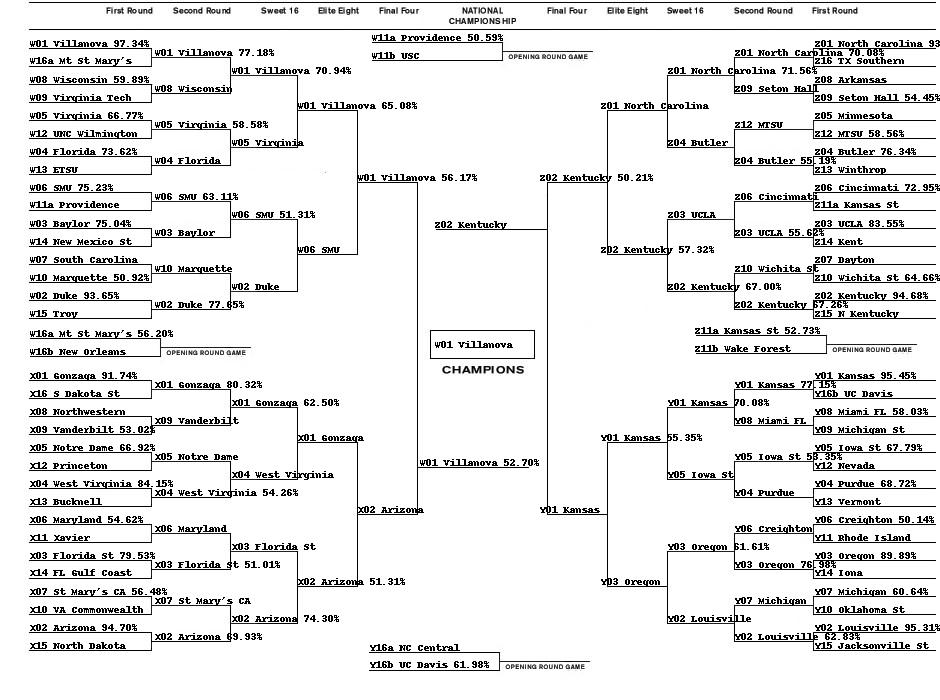
\includegraphics[width=1\textwidth]{bracket.jpg}

\newpage

\section{Evaluation of the Team}
\
\par Alex Hoffer has been the writer and GUI creator of the team. Alex build the primary website. Alex has also done most of the submitting our work.
\par Jake Smith collects the data and found a few helpful examples in helping Chongxian doing machine learning resarch.
\par Chongxian Chen has been the technical expert doing the python script of machine learning and editing it to allow user selection of stats. I have also wrote a simple php script to allow the user choose different stats to consider. I also set up the AWS server and put our project script on it.
\par I believe Alex and Jake has done equally important work as I have done. We function well as a team and are able to finish the requirements and responsibilities very well. 

\end{document}
